Un ordinateur est un dispositif complexe, qui consiste en de nombreux niveaux
d'abstraction.

\todo{citer Tanenbaum}

\cite{tanenbaum}

% Fig Archi {{{
\todo{À vérifier / mettre à jour}

\begin{figure}
\centering
\begin{tikzpicture}
[ every node/.style={}
, node distance=2cm
]

\node (cpu) {CPU};

\node[below of=cpu] (northb) {Northbridge};

\node[right of=northb] (mem) {Mémoire};
\node[left of=northb]  (agp) {AGP};
\node[below of=northb] (southb) {Southbridge};

\node[below left of=southb, xshift=-1cm] (sata) {SATA};
\node[below right of=southb, xshift=1cm] (usb)  {USB};

\node[below left of=sata]  (hdd)     {Disque dur};
\node[below right of=sata] (cdrom)   {CD-ROM};

\node[below left of=usb]  (memo)    {Mémorette};
\node[below right of=usb] (clavier) {Clavier};

\draw (cpu) -- (northb);
\draw (northb) -- (agp);
\draw (northb) -- (mem);
\draw (southb) -- (northb);
\draw (southb) -- (sata);
\draw (southb) -- (usb);
\draw (usb) -- (memo);
\draw (usb) -- (clavier);
\draw (sata) -- (hdd);
\draw (sata) -- (cdrom);

\end{tikzpicture}

\caption{Architecture simplifiée d'un ordinateur}
\label{fig:archi-simplifiee}
\end{figure}
% }}}

Au plus bas, il est constitué de nombreux composants matériels :
micro-processeur, mémoire, et divers périphériques
(figure~\ref{fig:archi-simplifiee}). Et au niveau de l'utilisateur, de dizaines
de logiciels permettant d'effectuer toutes sortes de calculs et de
communication.

Au cours de l'histoire des systèmes informatiques, la manière de les programmer
a beaucoup évolué. Au départ, les programmeurs avaient accès au matériel dans
son intégralité : toute la mémoire pouvait être accédé, toutes les instructions
pouvaient être utilisées.

Néanmoins c'est un peu restrictif : si on est seul à utiliser un système, on est
par définition... seul à pouvoir l'utiliser. Dans la seconde moitié des années
60, sont apparus les premiers systèmes "à temps partagé", permettant à plusieurs
utilisateurs de travailler en même temps.

Permettre l'exécution de plusieurs programmes en même temps est une idée
révolutionnaire, mais elle n'est pas sans difficultés techniques : en effet les
resources de la machine doivent être aussi partagées entre les utilisateurs et
les programmes. Par exemple, plusieurs programmes vont par exemple utiliser le
CPU les uns à la suite des autres (partage \emph{temporel}) ; et chaque
programme aura à sa disposition une partie de la mémoire principale, ou du
disque dur (partage \emph{spatial}).

Si deux programmes (ou plus) s'exécutent de manière concurrente sur le même
matériel, il faut s'assurer par exemple que les deux s'exécutent à peu près
aussi souvent, ou que l'un ne puisse pas écrire dans la mémoire de l'autre. Ce
sont des rôles du système d'exploitation.

Cela passe donc par un certain bridage des possibilités du programme : plutôt
que de le faire exécuter n'importe quel type d'instruction, il communique avec
le système d'exploitation. Bien que cela ait l'air d'une limitation, c'est aussi
bénéfique pour le programmeur puisque cela permet de définir des abstractions au
niveau du noyau.

Par exemple, si un programmeur veut copier des données depuis un CD-ROM vers la
mémoire principale, il devra interroger le bus SATA, interroger le lecteur sur
la présence d'un disque dans le lecteur, activer le moteur, calculer le numéro
de \emph{frame} des données sur le disque, demander la lecture, puis déclencher
une copie de la mémoire.

Si dans un autre cas il voulait récupérer des données depuis une mémorette USB,
il devrait interroger le bus USB, rechercher le bon numéro de périphérique, le
bon \emph{endpoint} dans celui-ci, lui appliquer une commande de lecture au bon
numéro de bloc, puis copier la mémoire.

Ces deux opérations, bien qu'elles aient le même but (copier de la mémoire
depuis un périphérique amovible), ne sont pas effectuées en pratique de la même
manière. C'est pourquoi le système d'exploitation fournit les notions de
fichier, lecteur, etc : le programmeur n'a plus qu'à utiliser des commandes de
haut niveau (``monter un lecteur'', ``ouvrir un fichier'', ``lire dans un
fichier'') et selon le type de lecteur, le système d'exploitation effectuera les
actions appropriées.

En résumé, un système d'exploitation est l''intermédiaire entre le logiciel et
le matériel, et en particulier assure les rôles suivants :

\begin{itemize}
\item gestion des processus : un système d'exploitation peut permettre
  d'exécuter plusieurs programme à la fois. Il faut alors orchestrer ces
  différents processus et les séparer en terme de temps et de ressources
  partagées.
\item
  gestion de la mémoire : chaque processus, en plus du noyau, doit disposer d'un
  espace mémoire différent. C'est-à-dire qu'un processus ne doit pas pouvoir
  interférer avec un autre.
\item
  gestion des périphériques : le noyau étant le seul code à s'exécuter en mode
  privilégié, c'est lui qui doit communiquer avec les périphériques matériels.
\item
  abstractions : le noyau fournit au programmes une interface unifiée,
  permettant de stocker des informations de la même manière sur un disque dur ou
  une clef USB (alors que l'accès se déroulera de manière très différente en
  pratique). C'est ici que la notion arbitraire de fichier sera définie, par exemple.
\end{itemize}

\section{Contexte}

Une description plus détaillée de l'implantation de Linux peut être trouvée dans
\cite{UnderstandingTheLinuxKernel}.

\section{Rôle d'un système d'exploitation}
\section{Espace noyau, espace utilisateur}

\todo{OS = kernel ?}

Le système d'exploitation est l'interface logicielle entre le matériel et les
programmes qui vont s'exécuter sur un ordinateur. Pour une description détaillée
de son rôle typique, le lecteur pourra se référer à 

Néanmoins on peut citer les rôles suivants :


\section{Cas de Linux}

Sous Linux, on retrouve cette séparation entre espace noyau et espace
utilisateur. Cette section décrit l'implémentation de cette séparation dans le
contexte suivant :

\begin{itemize}
\item l'architecture Intel x86
\item un système 32 bits
\item le noyau Linux
\end{itemize}

Sous d'autres architectures et d'autres systèmes d'exploitation, des mécanismes
similaires existent, et ces travaux peuvent sans doute s'y appliquer.

L'isolation est réalisée par le matériel. Ce document présente le cas d'un
système Intel 32 bits (x86), mais sous d'autres architectures des protections
similaires existent.

Le processeur permet d'exécuter des tâches selon plusieurs niveaux de privilège,
aussi appellés \emph{rings} : du \emph{ring} 3, le moins privilégié, jusqu'au
\emph{ring} 0, le plus privilégié. On peut configurer le processeur de manière à
ce que les instructions privilégiées (accès aux ports d'entrée/sortie...) ne
soient possibles qu'en \emph{ring} 0. Bien que 4 niveaux soient disponibles,
Linux n'utilise que les \emph{rings} 0 et 3.

Cela profite également au concept de mémoire virtuelle : comme différentes
tâches vont avoir une vue de la mémoire différente, on peut réserver une zone de
la mémoire aux tâches privilégiées.

\begin{figure}

\begin{Verbatim}
+-------------------------------------+
|   Ring 3                            |
|                                     |
|       Programmes utilisateur        |
|                                     |
|                                     |
|   ^ | appels système                |
+---|-v-------------------------------+
|                                     |
|   Ring 0                            |
|                                     |
|       Noyau                         |
|                                     |
|   ^ | instructions privilégiées     |
+---|-v-------------------------------+

   Hardware
\end{Verbatim}

\begin{tikzpicture}

\begin{scope}

  %\path[clip] (0, 0.8) rectangle (5, -0.8);

  \foreach \x/\c in { 4/20, 3/30, 2/40, 1/50, 0/60 }
  \draw[fill=black!\c] ($ (-2,0) + (\x,0) $) circle (2 cm);

\end{scope}

%\draw [<-] (3.5, 0) -- ++(0,-2) node {Applications};
%\draw [<-] (0, 0) -- ++(0,-2) node {Noyau};

\end{tikzpicture}


\caption{Les différents \emph{rings}. Seul le \emph{ring} 0 a accès au hardware
via des instructions privilégiées. Pour accéder aux fonctionnalités du noyau,
les programmes utilisateur doivent passer par des appels système.}

\label{fig:rings}
\end{figure}

\begin{figure}
\centering
\fbox{
  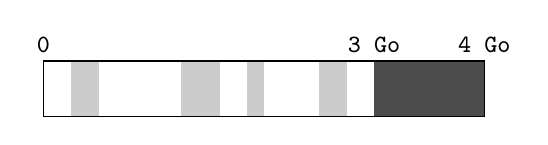
\begin{tikzpicture}
  [scale=0.7
  ,user/.style={fill=black!20}
  ,kernel/.style={fill=black!70}
  ]

  % Memory zone
  %
  % #1 - start
  % #2 - end
  % #3 - color
  \newcommand{\mzone}[3]{
    \path[#3] (#1,0) rectangle (#2,1);
  }

  % Address label
  %
  % #1 - x position
  % #2 - text
  \newcommand{\alabel}[2]{
    \path (#1,1) -- ++(0,0.3) node [pos=1] {\small \tt #2};

  }

  % exec
  \mzone{0.5}{1}{user}

  % lib
  \mzone{2.5}{3.2}{user}

  % stack
  \mzone{3.7}{4}{user}

  % stack
  \mzone{5}{5.5}{user}

  % kernel
  \mzone{6}{8}{kernel}

  % contour
  \draw (0,0) rectangle (8,1);

  \alabel{0}{0}
  \alabel{6}{3 Go}
  \alabel{8}{4 Go}

\end{tikzpicture}

}

\caption{L'espace d'adressage d'un processus. En gris clair, les zones
accessibles à tous les niveaux de privilèges : code du programme, bibliothèques,
tas, pile. En gris foncé, la mémoire du noyau, réservée au mode privilégié.}

\label{fig:memmap}
\end{figure}

\section{Appels système}

Les programmes utilisateur s'exécutant en \emph{ring} 3, ils ne peuvent pas
contenir d'instructions privilégiées, et donc ne peuvent pas accéder directement
au matériel (c'était le but !). Pour qu'ils puissent interagir avec le système
(afficher une sortie, écrire sur le disque...), le mécanisme des appels système
est nécessaire. Il s'agit d'une interface de haut entre les \emph{rings} 3 et 0.
Du point de vue du programmeur, il s'agit d'un ensemble de fonctions C
``magiques'' qui font appel au système d'exploitation pour effectuer des
opérations.

Prenons le cas de l'appel \texttt{getpid}, qui retourne le numéro de processus
courant. La bibliothèque C fournit une fonction du même nom :

\begin{center}\rule{3in}{0.4pt}\end{center}
\begin{Verbatim}
$ man getpid

GETPID(2)                  Linux Programmer's Manual                 GETPID(2)

NAME
       getpid, getppid - get process identification

SYNOPSIS
       #include <sys/types.h>
       #include <unistd.h>

       pid_t getpid(void);
       pid_t getppid(void);

DESCRIPTION

       getpid() returns the process ID of the calling process.  (This is often
       used by routines that generate unique temporary filenames.)
\end{Verbatim}
\begin{center}\rule{3in}{0.4pt}\end{center}

A priori, rien de différent d'une fonction implantée directement en C. Par un
processus détaillé ci-après, cette fonction va invoquer la fonction, suivante,
définie dans le noyau (\texttt{kernel/timer.c}) :

\begin{Verbatim}
SYSCALL_DEFINE0(getpid)
{
        return task_tgid_vnr(current);
}
\end{Verbatim}

Le mécanisme de couplage entre ces deux fonctions est le suivant :

\begin{itemize}
\item
  la fonction de la libc place les arguments éventuels de l'appel
  système dans les registres.
\item
  un numéro identifiant l'appel système est placé dans \eax.
\item
  une interruption logicielle est déclenchée :
\item
  l'exécution continue en \emph{ring} 0, à un point d'entrée prédéfini.
\item 
  les registres sont placés sur la pile noyau
\item
  le noyau examine le numéro d'appel système (toujours dans \eax) et appelle la
  fonction correspondante (les arguments sont en place sur la pile)
\item
  à la fin de la fonction, la valeur de retour est placé comme à l'habitude dans
  \eax et un \texttt{iret} permet de repasser en mode utilisateur, juste après
  l'appel système.
\end{itemize}

\todo{citer la doc intel}

\cite{intelsys}

Dans le cas d'un appel système qui ne fait que renvoyer un nombre, il n'y a pas
de difficulté. En revanche, certains appels système (la majorité, en fait),
remplissent une structure avec leurs résultats :

\begin{center}\rule{3in}{0.4pt}\end{center}

\begin{verbatim}
$ man gettimeofday

GETTIMEOFDAY(2)            Linux Programmer's Manual           GETTIMEOFDAY(2)



NAME
       gettimeofday, settimeofday - get / set time

SYNOPSIS
       #include <sys/time.h>

       int gettimeofday(struct timeval *tv, struct timezone *tz);
       int settimeofday(const struct timeval *tv, const struct timezone *tz);

   Feature Test Macro Requirements for glibc (see feature_test_macros(7)):

       settimeofday(): _BSD_SOURCE

DESCRIPTION
       The  functions  gettimeofday()  and  settimeofday() can get and set the
       time as well as a timezone.  The tv argument is a  struct  timeval  (as
       specified in <sys/time.h>):

           struct timeval {
               time_t      tv_sec;     /* seconds */
               suseconds_t tv_usec;    /* microseconds */
           };

       and  gives  the number of seconds and microseconds since the Epoch (see
       time(2)).  The tz argument is a struct timezone:

           struct timezone {
               int tz_minuteswest;     /* minutes west of Greenwich */
               int tz_dsttime;         /* type of DST correction */
           };

       If either tv or tz is NULL, the corresponding structure is not  set  or
       returned.  (However, compilation warnings will result if tv is NULL.)

RETURN VALUE
       gettimeofday() and settimeofday() return 0 for success, or -1 for fail‐
       ure (in which case errno is set appropriately).
\end{verbatim}
\begin{center}\rule{3in}{0.4pt}\end{center}

Pour utiliser une telle fonction, l'utilisateur doit allouer lui même la
mémoire, sur la pile par exemple :

\begin{Verbatim}
struct timeval tv;
struct timezone tz;
int z = gettimeofday(&tv, &tz);
if (z == 0) {
    printf( "tv.tv_sec = %ld\ntv.tv_usec = %ld\n"
            "tz.tz_minuteswest = %d\ntz.tz_dsttime = %d\n",
             tv.tv_sec, tv.tv_usec,
             tz.tz_minuteswest, tz.tz_dsttime
          );
}
\end{Verbatim}

Notons que dans ce cas, c'est le noyau qui remplit la structure : le
déréférencement se fait en \emph{ring} 0.
